%!TEX root = ../../dokumentation.tex

\chapter{Theoretische Grundlagen}
\label{chap:grundlagen}

Das folgende Kapitel bietet einen Überblick über den aktuellen Stand der Forschung und aktuelle Entwicklungen im Themenbereich des Cloud Computing und im Speziellen der Cloud Migration.

\section{Cloud Computing}

Im folgenden Unterkapitel werden die Grundlagen und eine Definition des Cloud Computing erarbeitet. Hierbei werden die Grundlegenden Konzepte, Bereitstellungsmodelle und Abstraktionsebenen des Cloud Computing erläutert.

\subsection{Was ist Cloud Computing}

Nach dem \ac{NIST}, auf dessen Definition sich in jüngerer Literatur häufig bezogen wird \cite[Vgl.][S. 4f]{Reinheimer2018}, ist Cloud Computing ein Modell der Zurverfügungstellung von Computing Ressourcen (z.B. Netzwerke, Server, Speicher, Anwendungen und Services),die über das Netzwerk erreichbar sind und mit geringem Managementaufwand schnell freigegeben und bereitgestellt werden können \cite[Vgl.][S. 2]{Mell2011}\cite[Vgl.][S. 5]{Reinheimer2018}.

\begin{wrapfigure}{r}{0.45\textwidth}
\centering
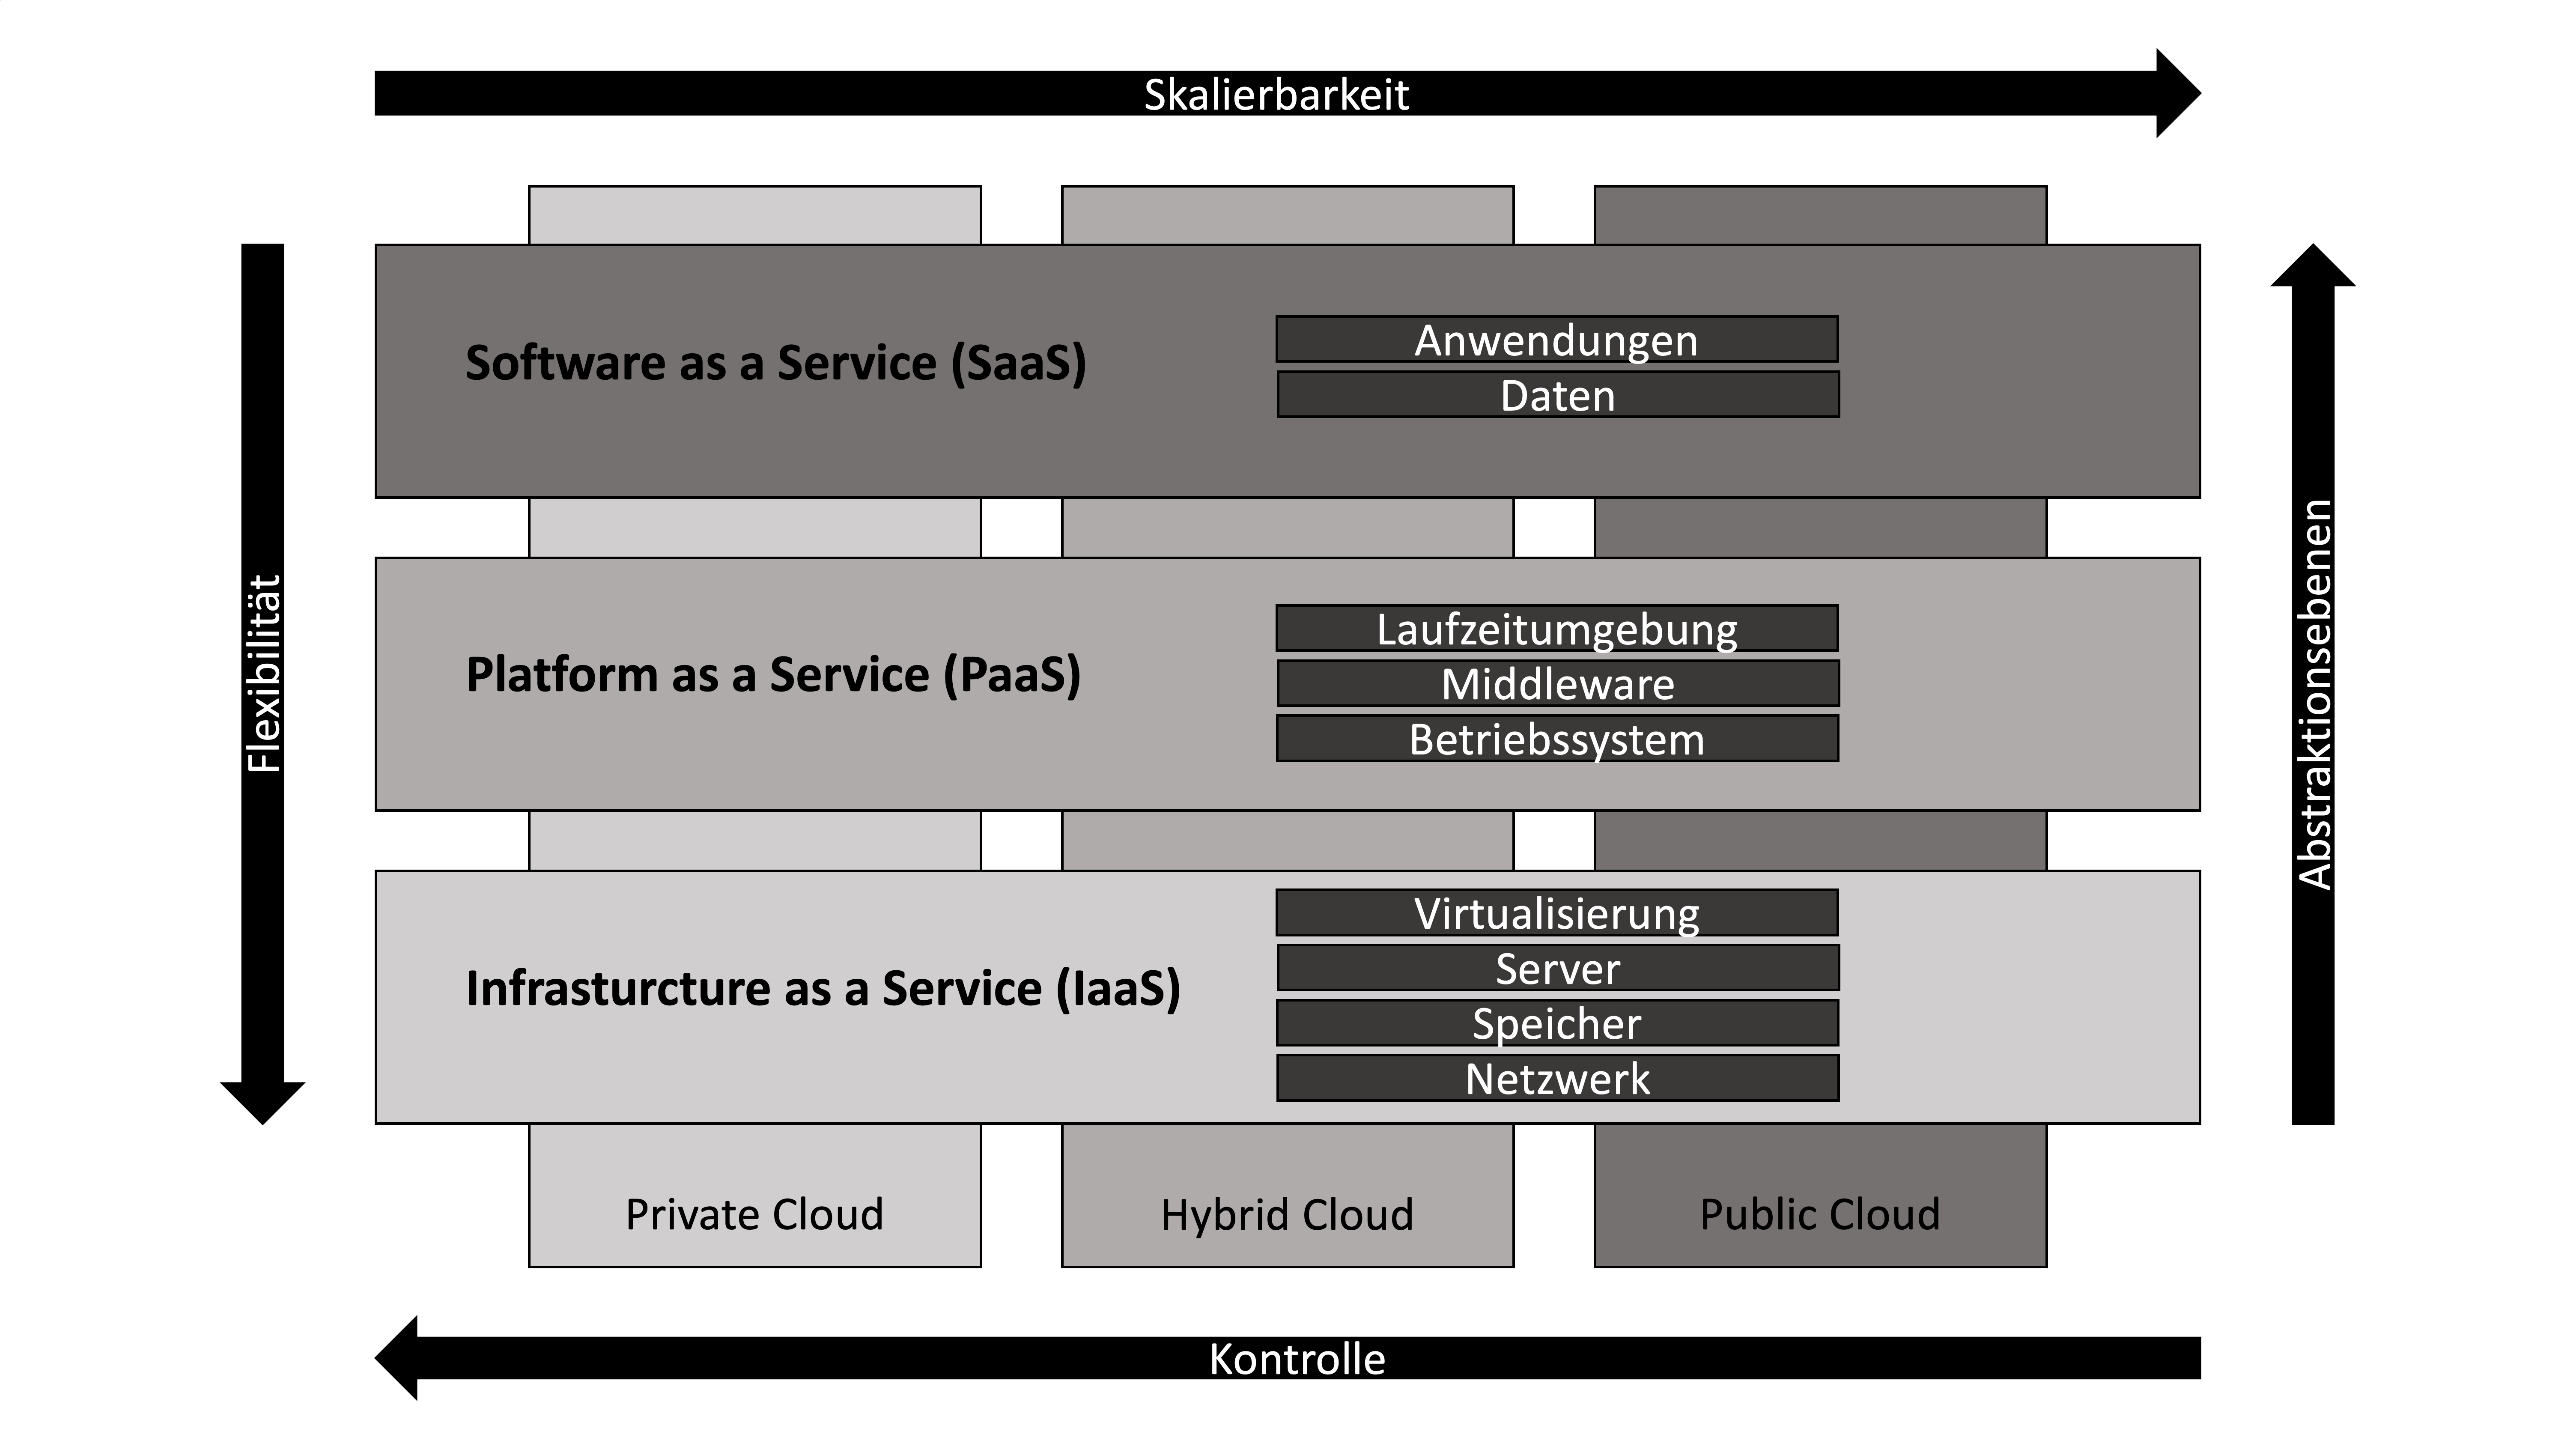
\includegraphics[height=0.3\textwidth]{xaas.png}
\caption{Eine Übersicht der Cloud Service Modelle \cite[Eigene Darstellung nach][S. 33]{Maenhaut2016}\cite[Ergänzt durch][]{Toroman2018}}
\label{fig:XaaS}
\end{wrapfigure}

Nach Hentschel und Leyh (2018), Zhao (2014), Maenhaut (2016) und Surianarayanan (2019) kann man Cloud Services grundsätzlich in drei Abstraktionsebenen einteilen. Diese sind \textbf{\ac{SaaS}}, \textbf{\ac{PaaS}} und \textbf{\ac{IaaS}}, welche auch zu \ac{XaaS} zusammengefasst werden \cite[Vgl.][S. 9]{Reinheimer2018}\cite[Vgl.][S. 143f]{Zhao2014}\cite[Vgl.][S. 32ff]{Maenhaut2016} und \cite[Vgl.][S. 226ff]{Surianarayanan2019}.

Die in Abbildung \ref{fig:XaaS} dargestellte unterste der drei genannten Abstraktionsschichten ist \ac{IaaS}, welche die Basisinfrastruktur, wie zum Beispiel Netzwerk, Server oder Speicher, bereitstellt.

Diese Infrastruktur kann sowohl physisch als auch virtuell zur Verfügung gestellt werden \cite[Vgl.][S. 9f]{Reinheimer2018}. Die darüberliegend dargestellte Schicht ist \ac{PaaS}, welche zu der Infrastrukturebene zusätzlich noch eine Basis zur Anwendungsentwicklung bietet, indem zum Beispiel bereits ein Betriebssystem und Middleware und eine Laufzeitumgebung bereitgestellt werden \cite[Vgl.][S. 10]{Reinheimer2018}. Die oberste Abstraktionsebene ist \ac{SaaS}, welche standardisierte Anwendungen zur Verfügung stellt und sich somit direkt an den Endnutzer richtet und ohne Verwaltung der zugrundeliegenden Ressourcen genutzt werden kann. Diese wird vom Provider übernommen.
\cite[Vgl.][S. 11]{Reinheimer2018}.

Generell wird die Cloud darüber hinaus in drei Organisationsdimensionen eingeteilt \cite[Vgl. auch im Folgenden][S. 7ff]{Reinheimer2018}:
\begin{itemize}
\item \textbf{Private Cloud:} Die Private Cloud bietet die exklusive Nutzung durch eine Organisation der darunterliegenden Infrastruktur. Die IT-Infrastruktur einer Private Cloud kann entweder im Unternehmenseigenen Rechenzentrum untergebracht oder auch von Dienstleistern bereitgestellt werden.
\item \textbf{Public Cloud:} In der Public Cloud ist die Infrastruktur für mehr Anwender zugänglich und muss geteilt werden. Dafür muss als Anwender oft auch nur für die tatsächlich genutzte Leistung gezahlt werden. Da die Infrastruktur jedoch gleichzeitig von vielen genutzt wird, ist zum Beispiel der Betrieb von sicherheitskritischen Anwendungen schwierig.
\item \textbf{Hybrid Cloud:} Die Hybrid Cloud bildet eine kombinierte Anwendung aus der Public Cloud und der Private Cloud. Diese bietet dem Anwender die Möglichkeit gewisse Anwendungen in die Public Cloud auszulagern, ohne die Vorteile der Private Cloud für sicherheitsrelevante Anwendungen aufgeben zu müssen. Darüber hinaus kann bei einem Hybrid Cloud Modell die Rechenleistung der Private Cloud bei Spitzenlast durch die Public Cloud erweitert werden. 
\end{itemize}

\pagebreak

\subsection{Entwicklung des Cloud Computing}

Die Entwicklung des Cloud Computing und dessen Vorgängerkonzepte is bis in die 90er Jahre zurückzuführen. Ein von Hentschel und Leyh (2018) hervorgehobener Vorgänger ist das sogenannte Grid Computing. Damit war bereits eine dezentrale Ressourcenkontrolle mir standardisierten Protokollen und Schnittstellen realisiert. Das Cloud Computing bietet vergleichbare Eigenschaften, jedoch rückt der Fokus hier auf wirtschaftliche Kriterien und die Zentralisierung von Ressourcen zum Beispiel in Rechenzentren \cite[Vgl.][S. 5f]{Reinheimer2018}.

Salesforce war eines der ersten Unternehmen, welches 1999 Anwendungen über eine Webseite bereitgestellt hat, gefolgt von den \ac{AWS} in 2002, welche Speicher und Rechenleistung als Services bereitstellten \cite[Vgl.][S. 17f]{Srivastava2018}.

\begin{figure}[h]
    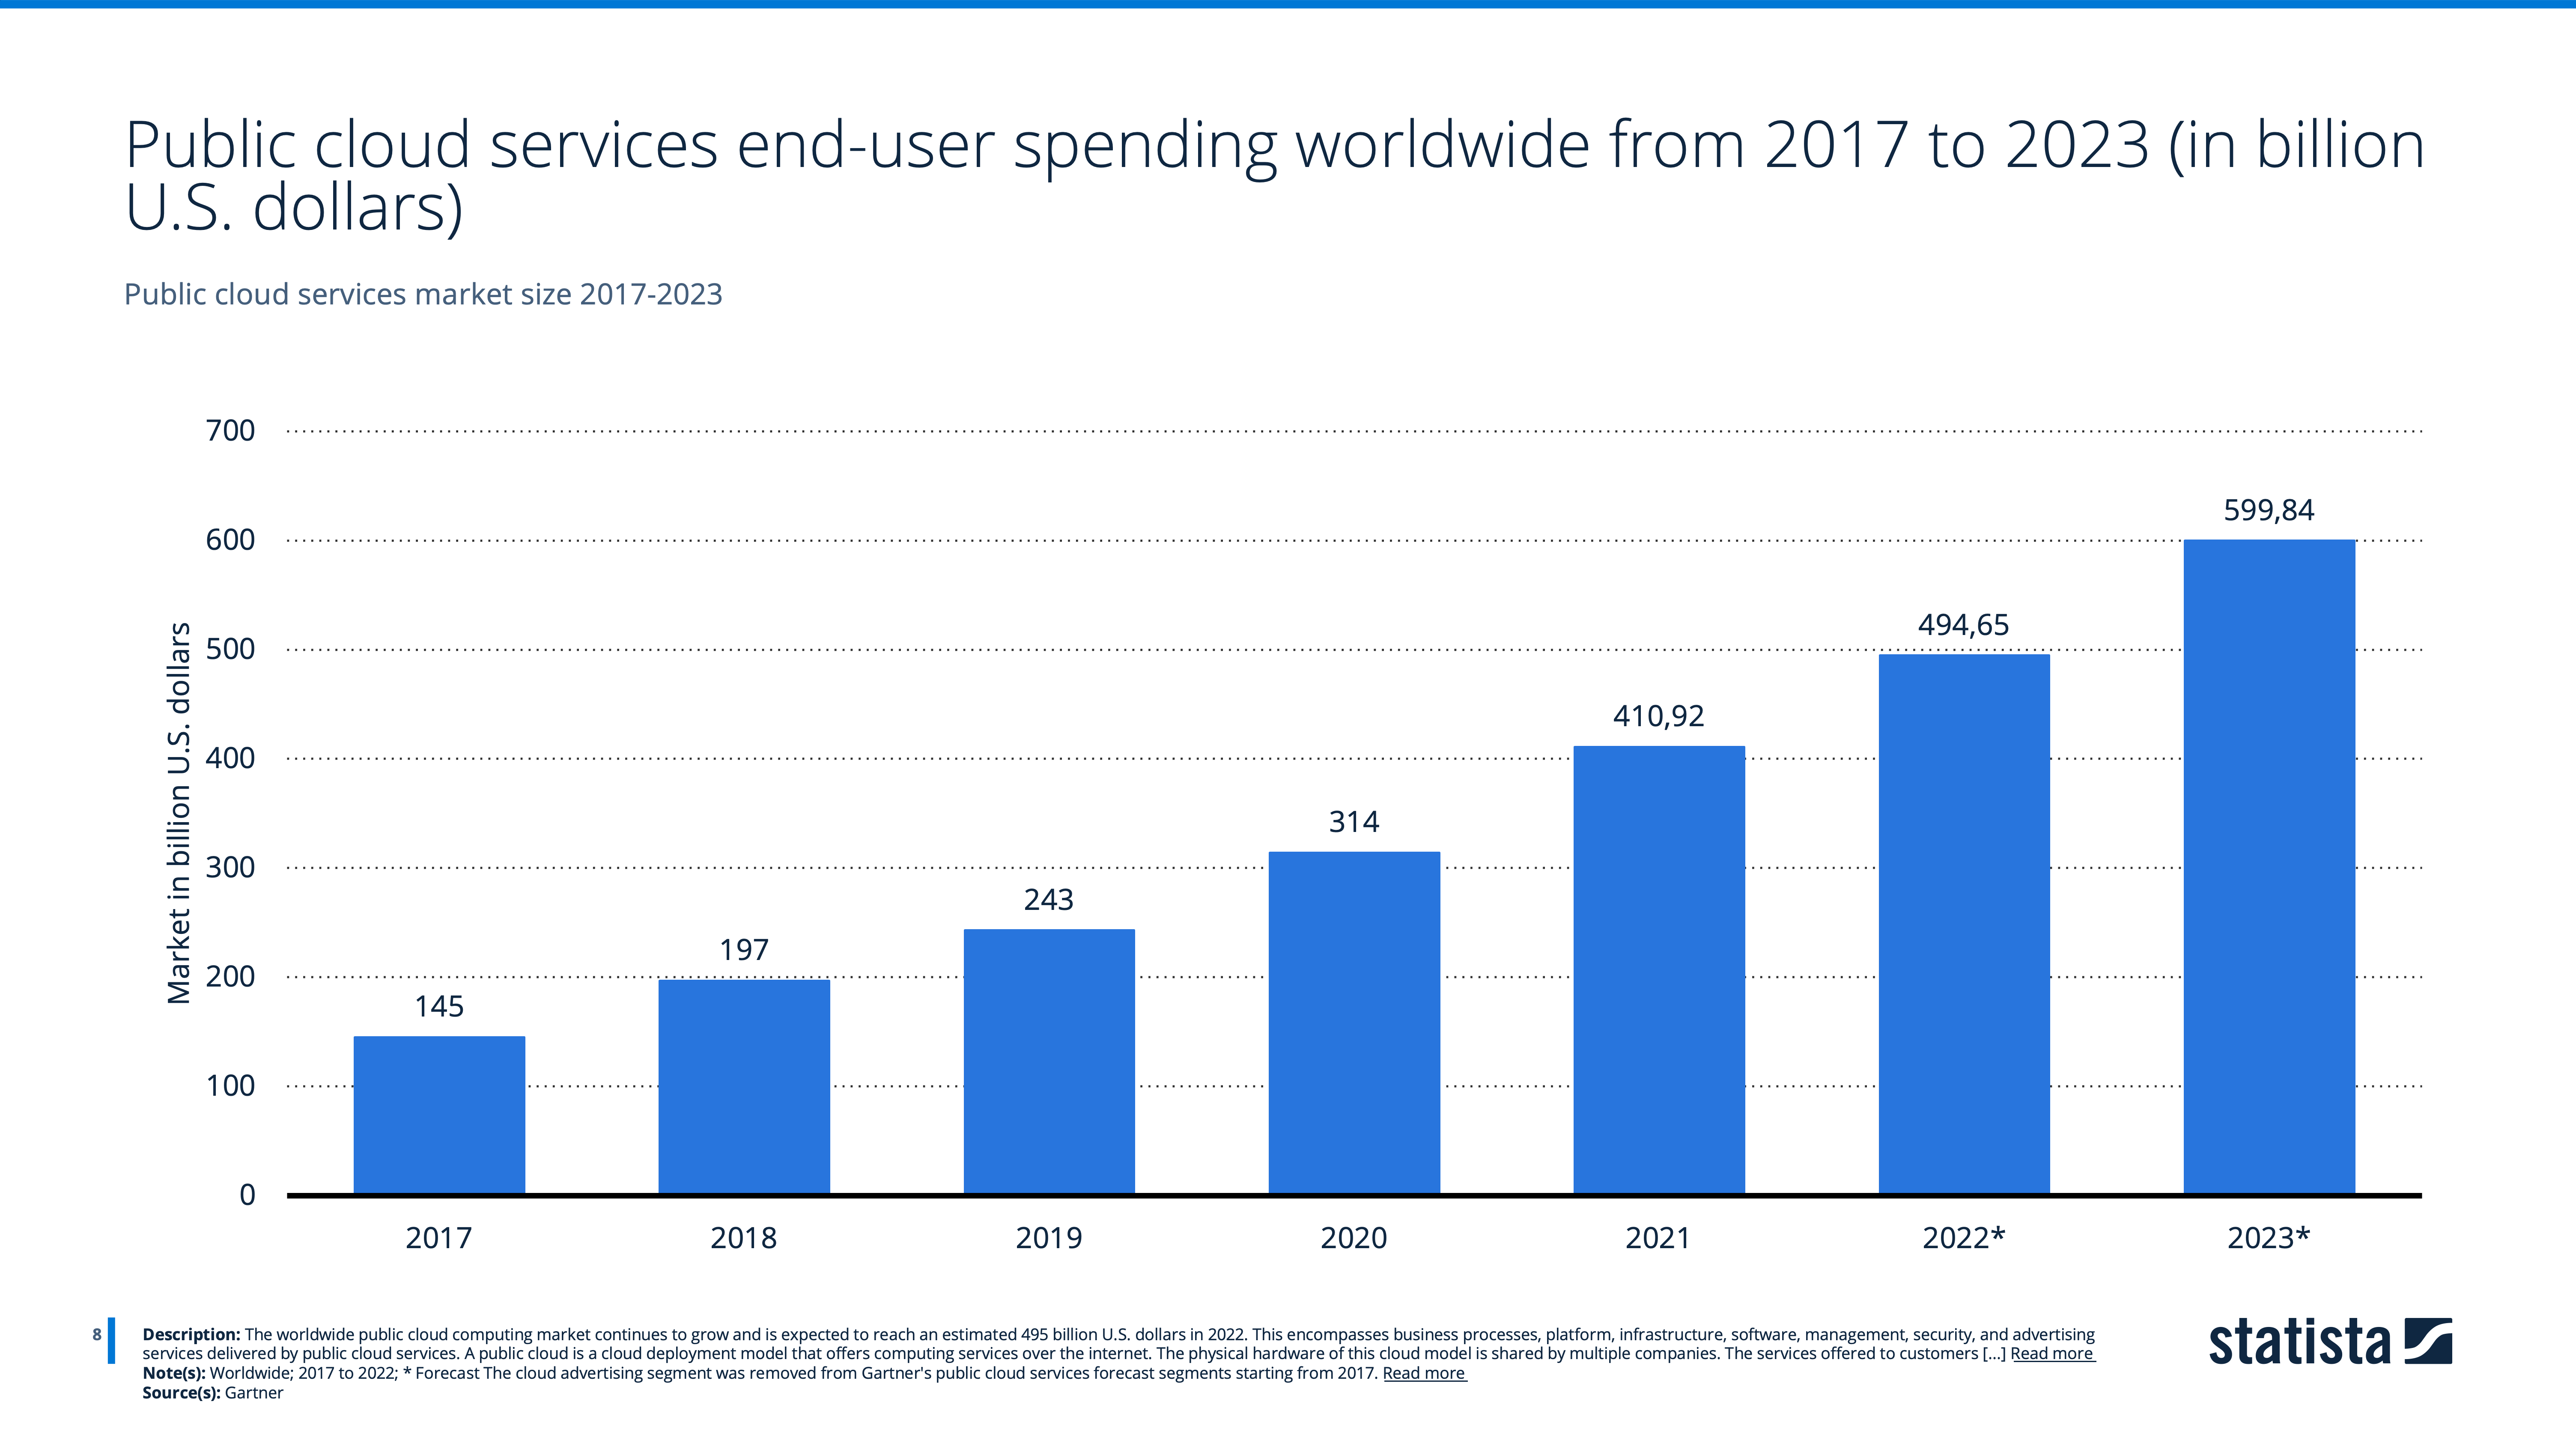
\includegraphics[width=\textwidth]{public_cloud_spending.png}
    \caption{Die Verkaufsleistungen der Public Cloud in den letzten Jahren \cite[S. 8]{Statista2022}}
    \label{fig:public_cloud_spending}
\end{figure}

Aus einem Dossier von Statista 2022 geht in der in Abbildung \ref{fig:public_cloud_spending} gezeigten Statistik hervor, dass sich die Ausgaben für public Cloud Services von 2017 bis 2023 etwas mehr als vervierfacht haben werden \cite[Vgl.][S. 8]{Statista2022}. Auch weitere Statistiken desselben Dossiers machen einen stetig steigenden Trend hinsichtlich des Cloud Computing deutlich \cite[Vgl. unter anderem][S. 11ff]{Statista2022}. 

\pagebreak

\subsection{Herausforderungen -> Migration von Legacy Anwendungen}

Neben der steigenden Nutzung von Cloud Computing und der Entwicklung Cloud basierter Anwendungen können auch legacy Anwendungen von Cloud Computing profitieren, woraus sich der trend abzeichnet, dass auch solche Anwendungen auf eine Cloud Infrastruktur migriert werden um die Ressourcen dieser nutzen zu können und Kosten zu sparen \cite[Vgl.][S. 31]{Maenhaut2016}.
\section{Merkmale von Cloud-Nativen Anwendungen}
\label{sec:cloud-native-anwendungen}
Mit Cloud-nativen Anwendungen kann das maximale Potenzial des Cloud Computing ausgenutzt werden \cite[Vgl.][]{VMwareb}. So können Produktivität und Effizienz gesteigert die Anwendungen schneller ausgeliefert werden \cite[Vgl][S. 12]{Chandrasekaran2022}. Im Folgenden werden die Merkmale von Cloud-nativen Anwendungen genauer untersucht.

% Was ist eine Cloud Native Anwendung?
% Merkmale
\subsection{Skalierbarkeit}
Von \textit{Cloud-native} Anwendungen wird unter anderem erwartet, dass diese schnell skalieren können, um unter anderem einer steigenden Nutzerzahl gerecht zu werden \cite[Vgl.][S. 1ff]{Armbrust2009} \cite[Vgl.][S. 234]{Villamizar2017}. Um die Vorteile der Cloud aber auch hinsichtlich der Kosten nutzen zu können, müssen die Services genauso herunter zu skalieren sein \cite[Vgl.][S. 884]{Adzic2017}.

Skalierbarkeit bedeutet in diesem Zusammenhang, dass die bereitgestellten IT-Ressourcen, wie Rechen- oder Speicherkapazität an die aktuelle Last angepasst werden können und entsprechen erhöht oder oder reduziert werden \cite[Vgl.][S. 15]{Reinheimer2018}\cite[Vgl.][]{Geißler2019}. Dabei wird in zwei Arten der Skalierung eines Systems unterschieden: \textbf{vertikale Skalierung} und \textbf{horizontale Skalierung} \cite[Vgl.][]{Geißler2019}\cite[Vgl.][]{VMware}

\begin{figure}[H]
    \centering
    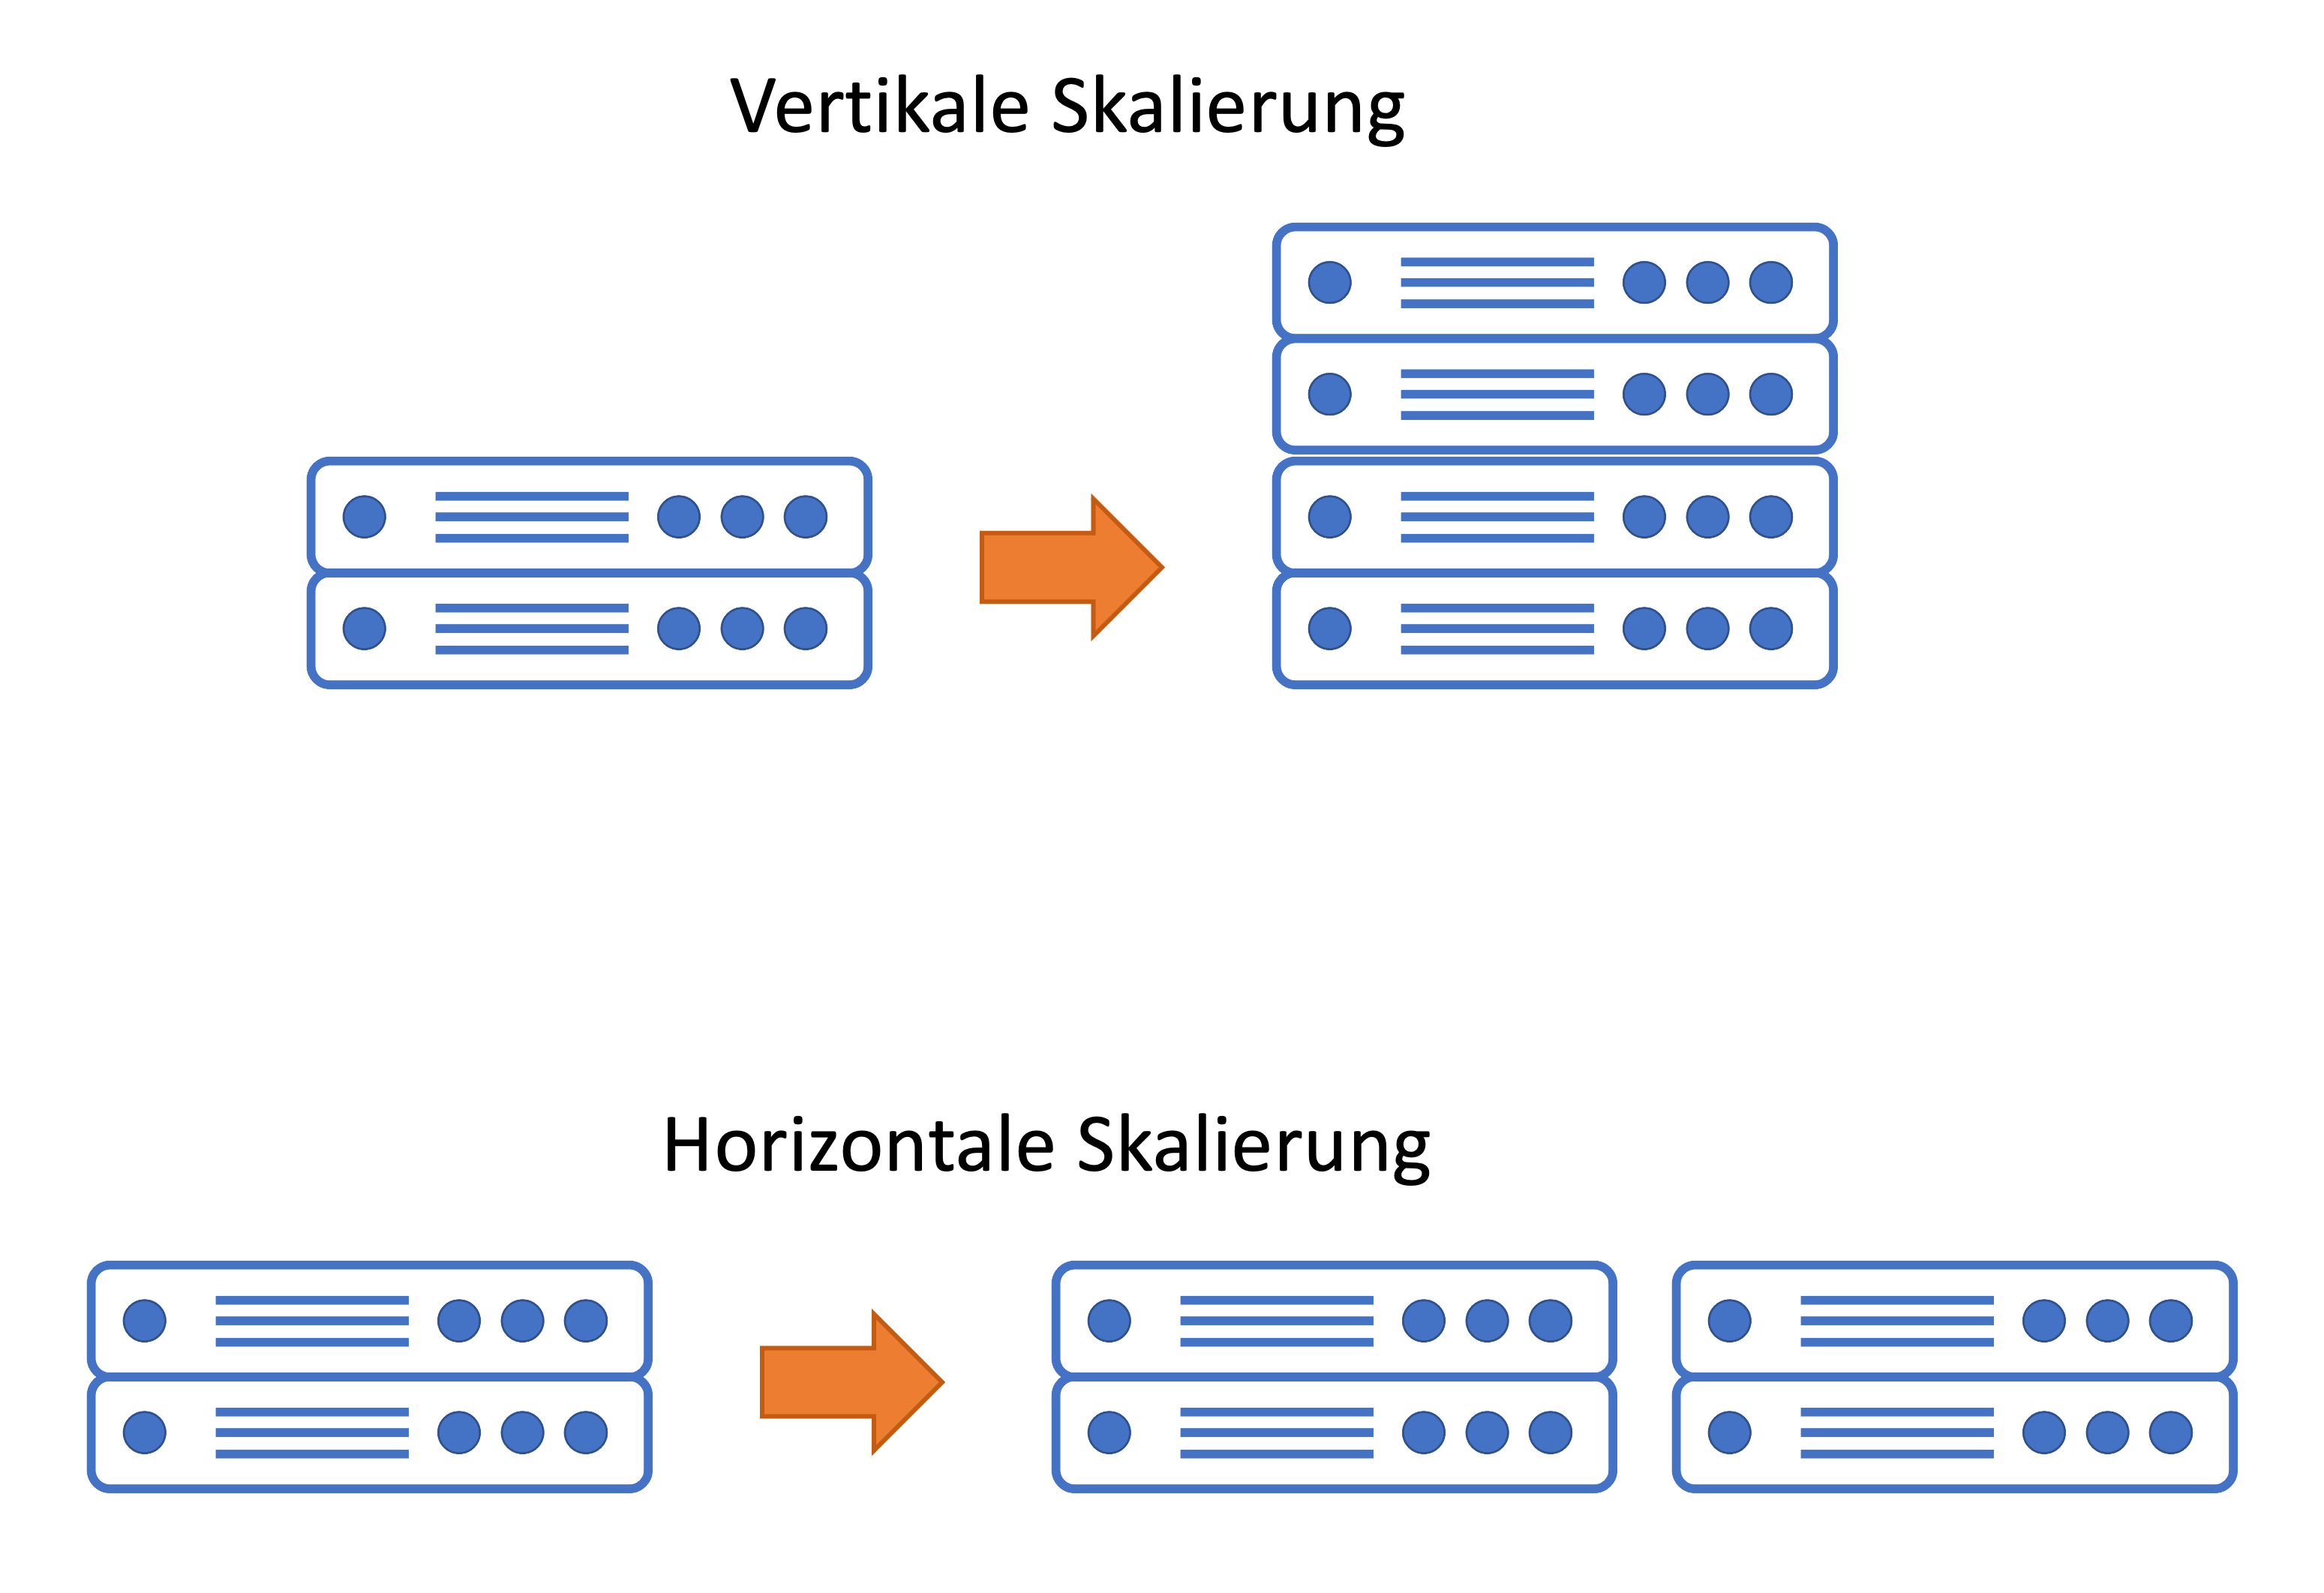
\includegraphics[width=0.65\textwidth]{scale-up_scale-out.png}
    \caption{Vertikale vs. Horizontale Skalierung \cite[Nachbildung nach][]{Bachmann2019}}
    \label{fig:scale-up-scale-out}
\end{figure}

\textbf{Vertikale Skalierung:}
Bei der vertikalen Skalierung wird zu einer Einheit innerhalb eines Systems zusätzliche Rechenleistung oder zusätzlicher Speicher hinzugefügt. Diese Art der Skalierung wird auch als ''Scale-up'' bezeichnet, abgeleitet von dem Erhöhen der Leistung. Die vertikale Skalierung ist jedoch dadurch limitiert, dass bei der Leistungsaufstockung hardwareseitig Grenzen gesetzt sind \cite[Vgl.][]{Geißler2019}\cite[Vgl.][]{VMware}. \pagebreak

\textbf{Horizontale Skalierung:}
Zur horizontalen Skalierung werden dagegen nicht die Ressourcen innerhalb einer Einheit erhöht, sondern weitere Einheiten beziehungsweise Knoten zu einem System hinzugefügt. Die Aufgaben werden dann auf mehreren Systemen durchgeführt, oder zum Beispiel eine Anwendung in mehreren Containern parallel ausgeführt. Horizontale Skalierung wird auch als ''Scale-out'' bezeichnet, da ein System hier in seiner Breite erweitert wird. In der Theorie sind der horizontalen Skalierung keine Grenzen gesetzt \cite[Vgl.][]{Geißler2019}\cite[Vgl.][]{VMware}.

\subsection{Fehlertoleranz}
Eine weitere Anforderung an Cloud-native Anwendungen ist die Fehlertoleranz. Es sollte grundsätzlich davon ausgegangen, dass Fehler auftreten können und diese abgefangen werden müssen \cite[Vgl.][S. 17]{Gannon2017}. Zu diesen Fehlern gehört unter anderem das Abstürzen von Container und Hardware- oder Netzwerkfehler.
% Auch durch horizontale Skalierung, weil einzelne Nodes ausfallen können

\subsection{Schnelle Bereitstellung}
Mit \textit{Continous Delivery}, zu deutsch kontinuierliche Bereitstellung, können Änderungen in der Anwendung unmittelbar ausgeliefert werden, ohne zum Beispiel auf ein Wartungsfenster nachts warten zu müssen oder die Änderungen mit weiteren Updates zu einem Release zu bündeln, bevor diese ausgeliefert werden \cite[Vgl.][]{VMwareb}.

\subsection{Containerisierung}
Gegenüber der Verwendung von \acp{VM} bieten Container eine höhere Effizienz und Geschwindigkeit. Das Starten und Beenden von Containern ist ein einer \ac{VM} zeitlich voraus. Darüber hinaus benötigt eine \ac{VM} weitere Pakete, da diese die Hardware virtualisiert, wogegen in Containern nur das Betriebssystem virtualisiert wird \cite[Vgl.][]{VMwareb}.

\subsection{Weitere Merkmale}
% Vorhersehbarkeit, kollaborative Entwicklung, Microservices
Weitere Merkmale Cloud-nativer Anwendungen sind unter anderem eine bessere Verlässlichkeit, durch eine gewährleistete ''Ausfallsicherheit'' und die Verwendung vieler unabhängiger Microservices (siehe Kapitel \ref{sec:architekturstile}), wodurch auch die Entwicklung in Teams erleichtert wird, da die Services unabhängig voneinander aktualisiert werden können \cite[Vgl.][]{VMwareb}.

\pagebreak
\section{Herausforderungen der Cloud Migration}
\label{sec:herausforderungen}

% Merkmale von Cloud nativen Anwendungen in legacy Applikationen umsetzen
% Verlass auf Box-API muss gegeben sein
% https://developers.redhat.com/articles/2021/06/14/application-modernization-patterns-apache-kafka-debezium-and-kubernetes#application_modernization_in_context

Cloud Computing birgt jedoch auch einige Herausforderungen, welche in der Entwicklung und Migration komplexe Aufgaben mit sich bringen können.

\subsection{Vorteile der Cloud nutzen}

Neben der steigenden Nutzung von Cloud Computing und der Entwicklung Cloud-basierter Anwendungen können auch \textit{legacy} Anwendungen von Cloud Computing profitieren. Daraus zeichnet sich der Trend ab, dass auch solche Anwendungen auf eine Cloud Infrastruktur migriert werden. Diese Entwicklung ermöglicht es, die Ressourcen der Cloud nutzen zu können und Kosten zu sparen \cite[Vgl.][S. 31]{Maenhaut2016}.

Abhängig vom gewählten Migrationsansatz sind Anpassungen in der Anwendung vorzunehmen, meist um die Vorteile der Cloud ausnutzen zu können. Verbesserung des Anwendungsdesigns und die Optimierung von Ressourcennutzung sind nach Feathers (2004) zwei der vier möglichen Hauptgründe Anpassungen an Software vorzunehmen \cite[Vgl.][S. 3]{Feathers2004}. Diese lassen sich auch auf die vorzunehmenden Anpassungen für eine Cloud Migration übertragen. Eine Herausforderung, die bei der Anpassung von Software aufkommt, ist es sicherzustellen das grundlegende Verhalten der Anwendungen nicht zu beeinträchtigen. Die Schwierigkeit liegt darin, oft nicht genau erkennen zu können, wie Stark das Verhalten der Anwendung auf diese Änderungen reagiert \cite[Vgl.][S. 7]{Feathers2004}. 

\subsection{Entwicklung von Cloud-basierten Anwendungen}

Eine weitere Herausforderung in der Anwendungsentwicklung ist, die Anwendung und den Entwicklungsprozess so zu gestalten, dass mehrere Entwickler gleichzeitig an verschiedenen Funktionen der Anwendung arbeiten können, ohne sich dabei gegenseitig in die Quere zu kommen. Auch darauf ist entsprechend bei der Cloud Migration von \textit{legacy} Anwendungen zu achten \cite[Vgl.][]{Ibryam2021}.

Außerdem wird im Zuge der Migration meist erwartet, dass die Vorteile der Cloud, wie zum Beispiel eine effiziente Skalierung der Anwendung, umgesetzt werden, was zusätzlichen Aufwand zur reinen Migration bedeutet \cite[Vgl.][]{Ibryam2021}. \pagebreak

\subsection{Datenschutz und Datensicherheit in der Cloud}
Personenbezogene und sensible (z. B. geschäftliche) Daten bedürfen einer guten Datensicherheit, vor allem im Kontext des Cloud Computing und dort insbesondere für die Public Cloud, wo Speicherressourcen nicht direkt in den Händen des Anwenders liegen, sondern in den Rechenzentren der Provider verarbeitet und gespeichert werden \cite[Vgl.][S. 1ff]{Sun2019}. Aus diesem Grund ist es wichtig, mögliche Risiken sowie die damit verbundenen Herausforderungen zu identifizieren \cite[Vgl.][S. 3]{Sun2019}.

Folgende Risiken können für Datenschutz und Datensicherheit in der Cloud existieren \cite[Vgl. auch im folgenden][S. 694]{Kumar2018}:

\begin{itemize}
    \item Risiken in Zusammenhang mit \textit{\ac{CIA}}\footnote{dt. Konsistenz, Integrität und Verfügbarkeit, }
    \item Herausforderungen bei der Authentifizierungs- und Zugriffskontrolle
    \item Fehlerhafte Authentifizierungs-, Sitzungs- und Zugriffskontrollen
    \item Weitere Risiken, die durch z. B. Speicherort der Daten, Mehrbenutzerfähigkeit oder Backups entstehen können
\end{itemize}

\pagebreak
\section{Migrationsansätze}
\label{sec:migrationsansaetze}

Im folgenden Kapitel wird auf die unterschiedlichen Migrationsmethoden des Cloud Computing eingegangen. Durch die unterschiedlichen Abstraktionsebenen bedingt gibt es verschiedene Ansätze, wie die Cloud Migration realisierbar ist \cite[Vgl.][S. 226]{Surianarayanan2019}, angefangen mit dem auch als \glqq{Lift and Shift}\grqq{} bezeichneten Rehosting, bis hin zur Migration zu \ac{SaaS} verbunden mit der Entwicklung Cloud nativer Anwendungen \cite[Vgl.][S. 144]{Zhao2014}.

\subsection{Migration zu IaaS (Rehosting)}
Nach Zhao (2014) ist vorallem das Rehosting die vorgeschlagene Strategie für die Migration zu \ac{IaaS} \cite[Vgl.][S. 144]{Zhao2014}. Umgangssprachlich wird diese Vorgehensweise auch als \glqq{Lift and Shift}\grqq{} bezeichnet \cite[Vgl.][]{NetApp}. Bei diesen Strategien werden Anwendungen lediglich auf einer anderen Hardwareplattform installiert, die Anwendungsarchitektur bleibt dabei unverändert. Dieser Ansatz bietet eine schnelle Lösung zur Migration \cite[Vgl.][]{CIO}.

Der wahrscheinlich größte Vorteil der Migration zu \ac{IaaS} ist, dass die Anwendungsarchitektur nicht verändert werden muss und die Migration somit schnell und ohne großen Aufwand vollzogen werden kann. Ein Nachteil ist dagegen, dass die Migration zu \ac{IaaS} nicht die vollen Möglichkeiten der Cloud ausnutzt.

\subsection{Migration zu PaaS (Refactoring/Rebuilding)}
Das Refactoring oder Rebuilding von Anwendungen gehört nach Zhao (2014) zu den empfohlenen Strategien für die Migration zu \ac{PaaS} \cite[Vgl.][S. 144]{Zhao2014}. Rebuilding bedeutet, den bisherigen Code zu re-architekten um die Vorteile der Cloud Plattform nutzen zu können \cite[Vgl.][]{CIO}. Darunter fällt zum Beispiel das Umsetzen entsprechender Service Topologien im Code \cite[Vgl.][S. 2]{Holmes2018}.

Durch die vom Cloud Provider teils vorgegebene Plattform (z.B. Middleware und Datenbanken) müssen Anwendungen dieser entsprechend angepasst werden \cite[Vgl.][S. 227]{Surianarayanan2019}. Der Mehrwert einer Migration zu \ac{PaaS} ist, dass der Anwender die IT-Infrastruktur nicht mehr managen muss und somit Aufwände reduziert werden können \cite[Vgl.][S. 6]{Pahl}.

\subsection{Migration zu SaaS (Cloud Native Entwicklung)}
Der Schritt zu \ac{SaaS} ist nach Zhao (2014) auf verschiedenen Wegen zu erreichen. Demnach sei eine Anwendung durch einen SaaS Service entweder zu ersetzen, entsprechend der SaaS Prinzipien zu überarbeiten oder zu einem \ac{SaaS} Service umzustrukturieren \cite[Vgl.][S. 144]{Zhao2014}.

Das Augeben einer Anwendung und vollständige Ersetzen dieser durch Nutzung des \ac{SaaS} Modells bedarf eines größeren Aufwand und ein Entwicklungsteam zur Umsetzung der Anforderungen \cite[Vgl.][]{CIO}.
\section{Architekturstile im Hintergrund des Cloud Computing}
\label{sec:architekturstile}
Die Architektur von Anwendungen ist in den meisten Fällen entweder monolithisch oder als Microservice Architektur umgesetzt \cite[Vgl.][S. 150]{Gos2020}. Das nachfolgende Kapitel beschreibt diese Architekturstile mit ihren Eigenschaften und aus welchem Grund die Microservice Architektur für den Betrieb in der Cloud bevorzugt eingesetzt wird \cite[Vgl.][S. 1]{Villamizar2015}.

\subsection{Monolithische Anwendungsarchitektur}
% Was sind monolithische Anwendungen?
Monolithische Anwendungen, wie sie in der Vergangenheit oft eingesetzt wurden, bestehen aus verschiedenen Komponenten, die zu einem Programm kombiniert werden. Die einzelnen Komponenten funktionieren nur zusammen innerhalb des Monolithen, einzelne Komponenten können also nicht unabhängig betrieben werden. \cite[Vgl.][S. 1]{Gos2020}.

\begin{figure}[H]
    \centering
    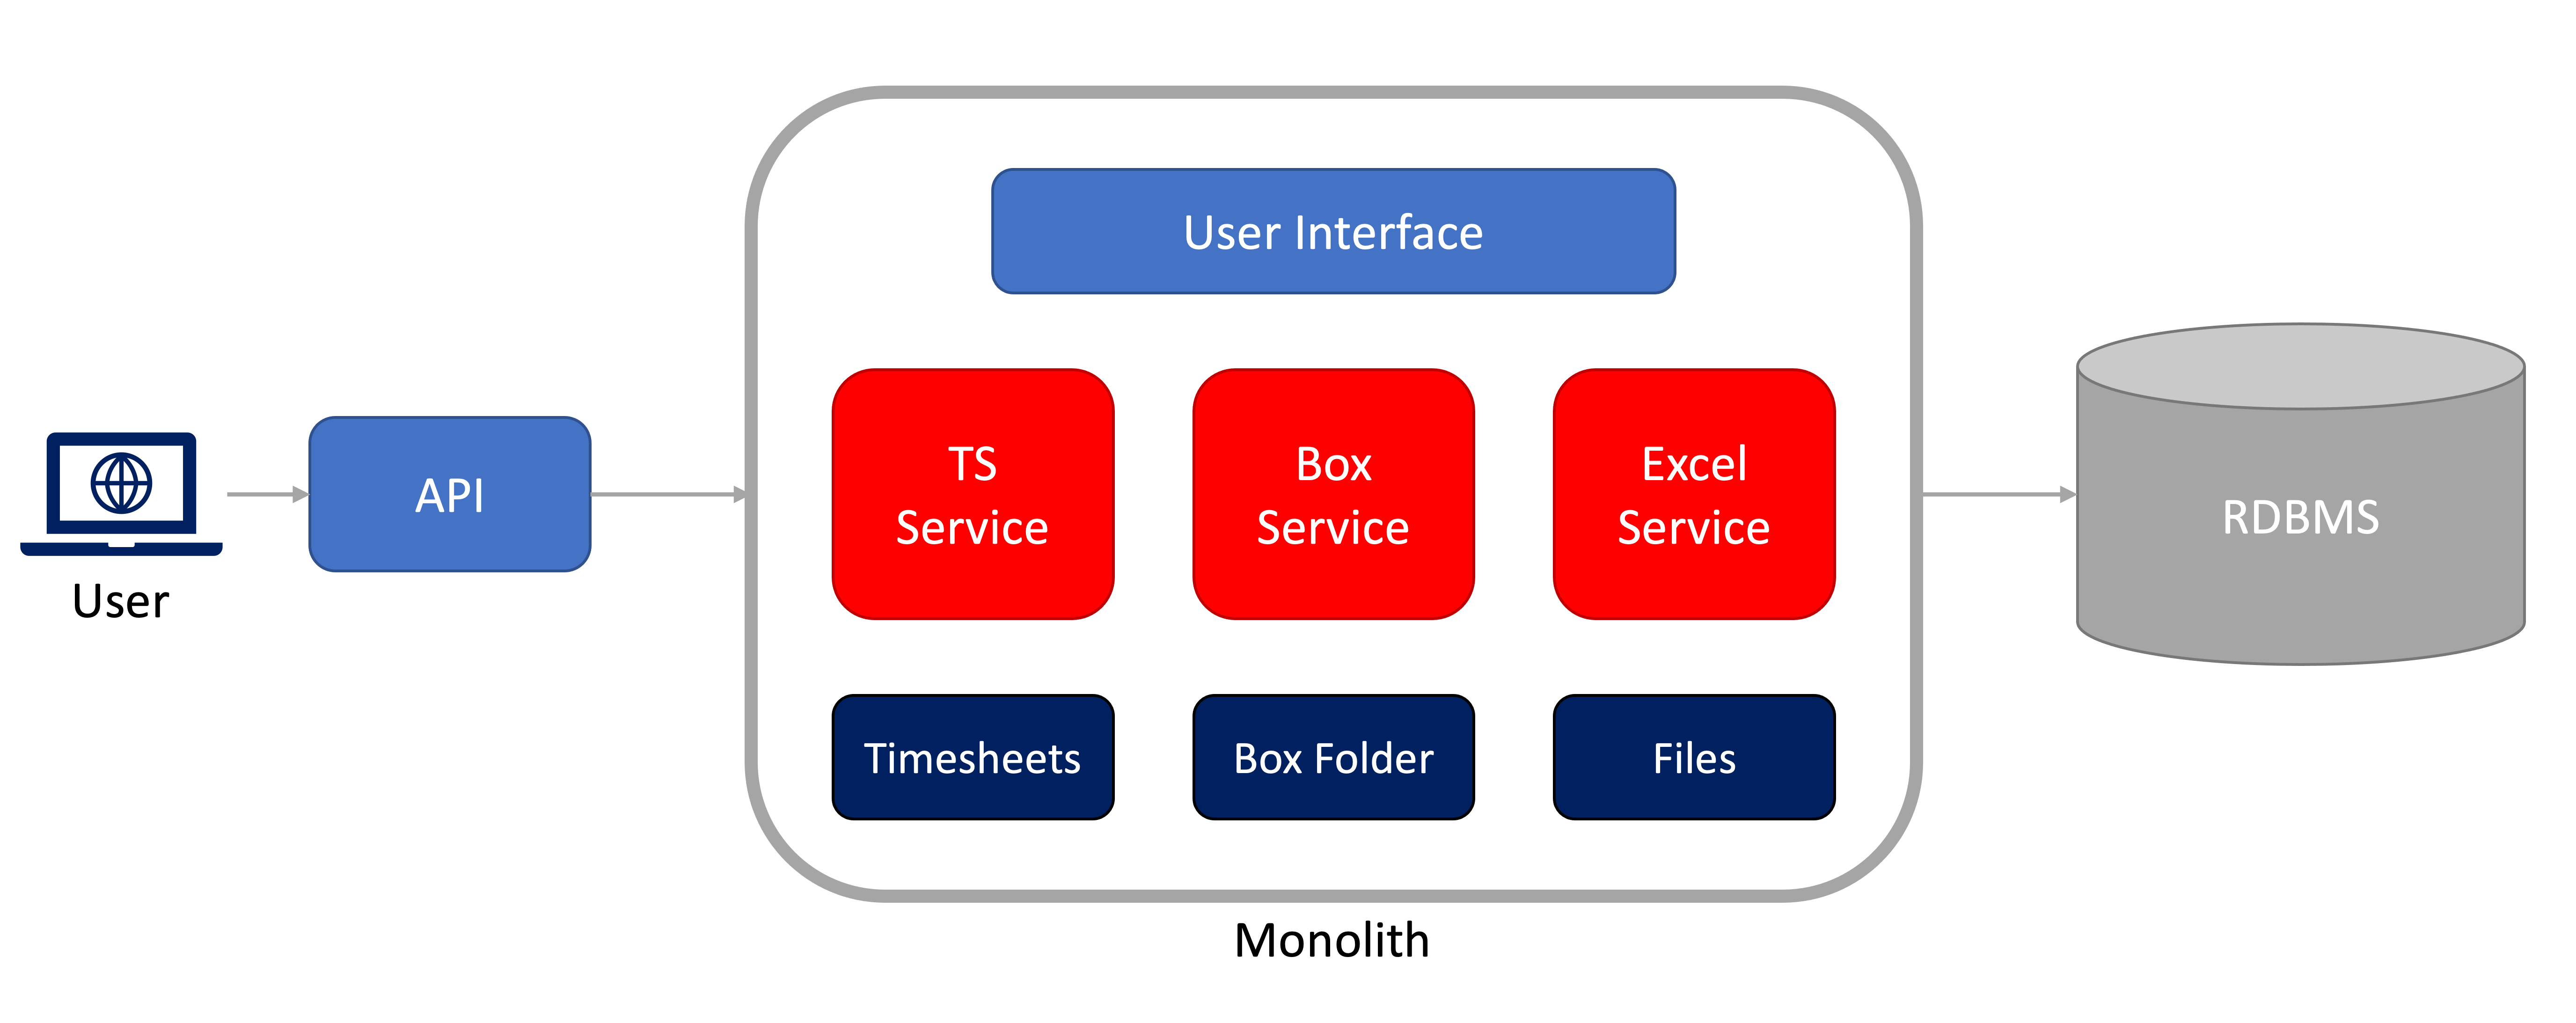
\includegraphics[width=0.65\textwidth]{monolith.png}
    \caption{Beispiel einer monolithischen Architektur \cite[Nachbildung angelehnt an][S. 150]{Gos2020}}
    \label{fig:monolith}
\end{figure}

Abbildung \ref{fig:monolith} zeigt, wie eine monolithische Architektur aufgebaut sein kann. Hier sind die Komponenten eng miteinander verwoben und voneinander abhängig.
% In Bezug auf Cloud Native -> warum nicht geeignet
\pagebreak

\subsection{Microservice Architektur}
Der Einsatz von Microservice Architekturen hat in den letzten Jahren stark zugenommen \cite[Vgl.][S. 150]{Gos2020}. Microservices bedeutet, dass eine Anwendung aus einer Zusammenstellung einzelner Services besteht, wobei jeder Service einen Teil der Business-Logik erfüllt. Diese Services sind dabei, wie in Abbildung \ref{fig:microservice} dargestellt voneinander unabhängig um keinen Single-Point of Failure zu erzeugen \cite[Vgl.][S. 150]{Gos2020}\cite[Vgl.][]{Janssen2021}\cite[Vgl.][]{Fowler2014}.

\begin{figure}[H]
    \centering
    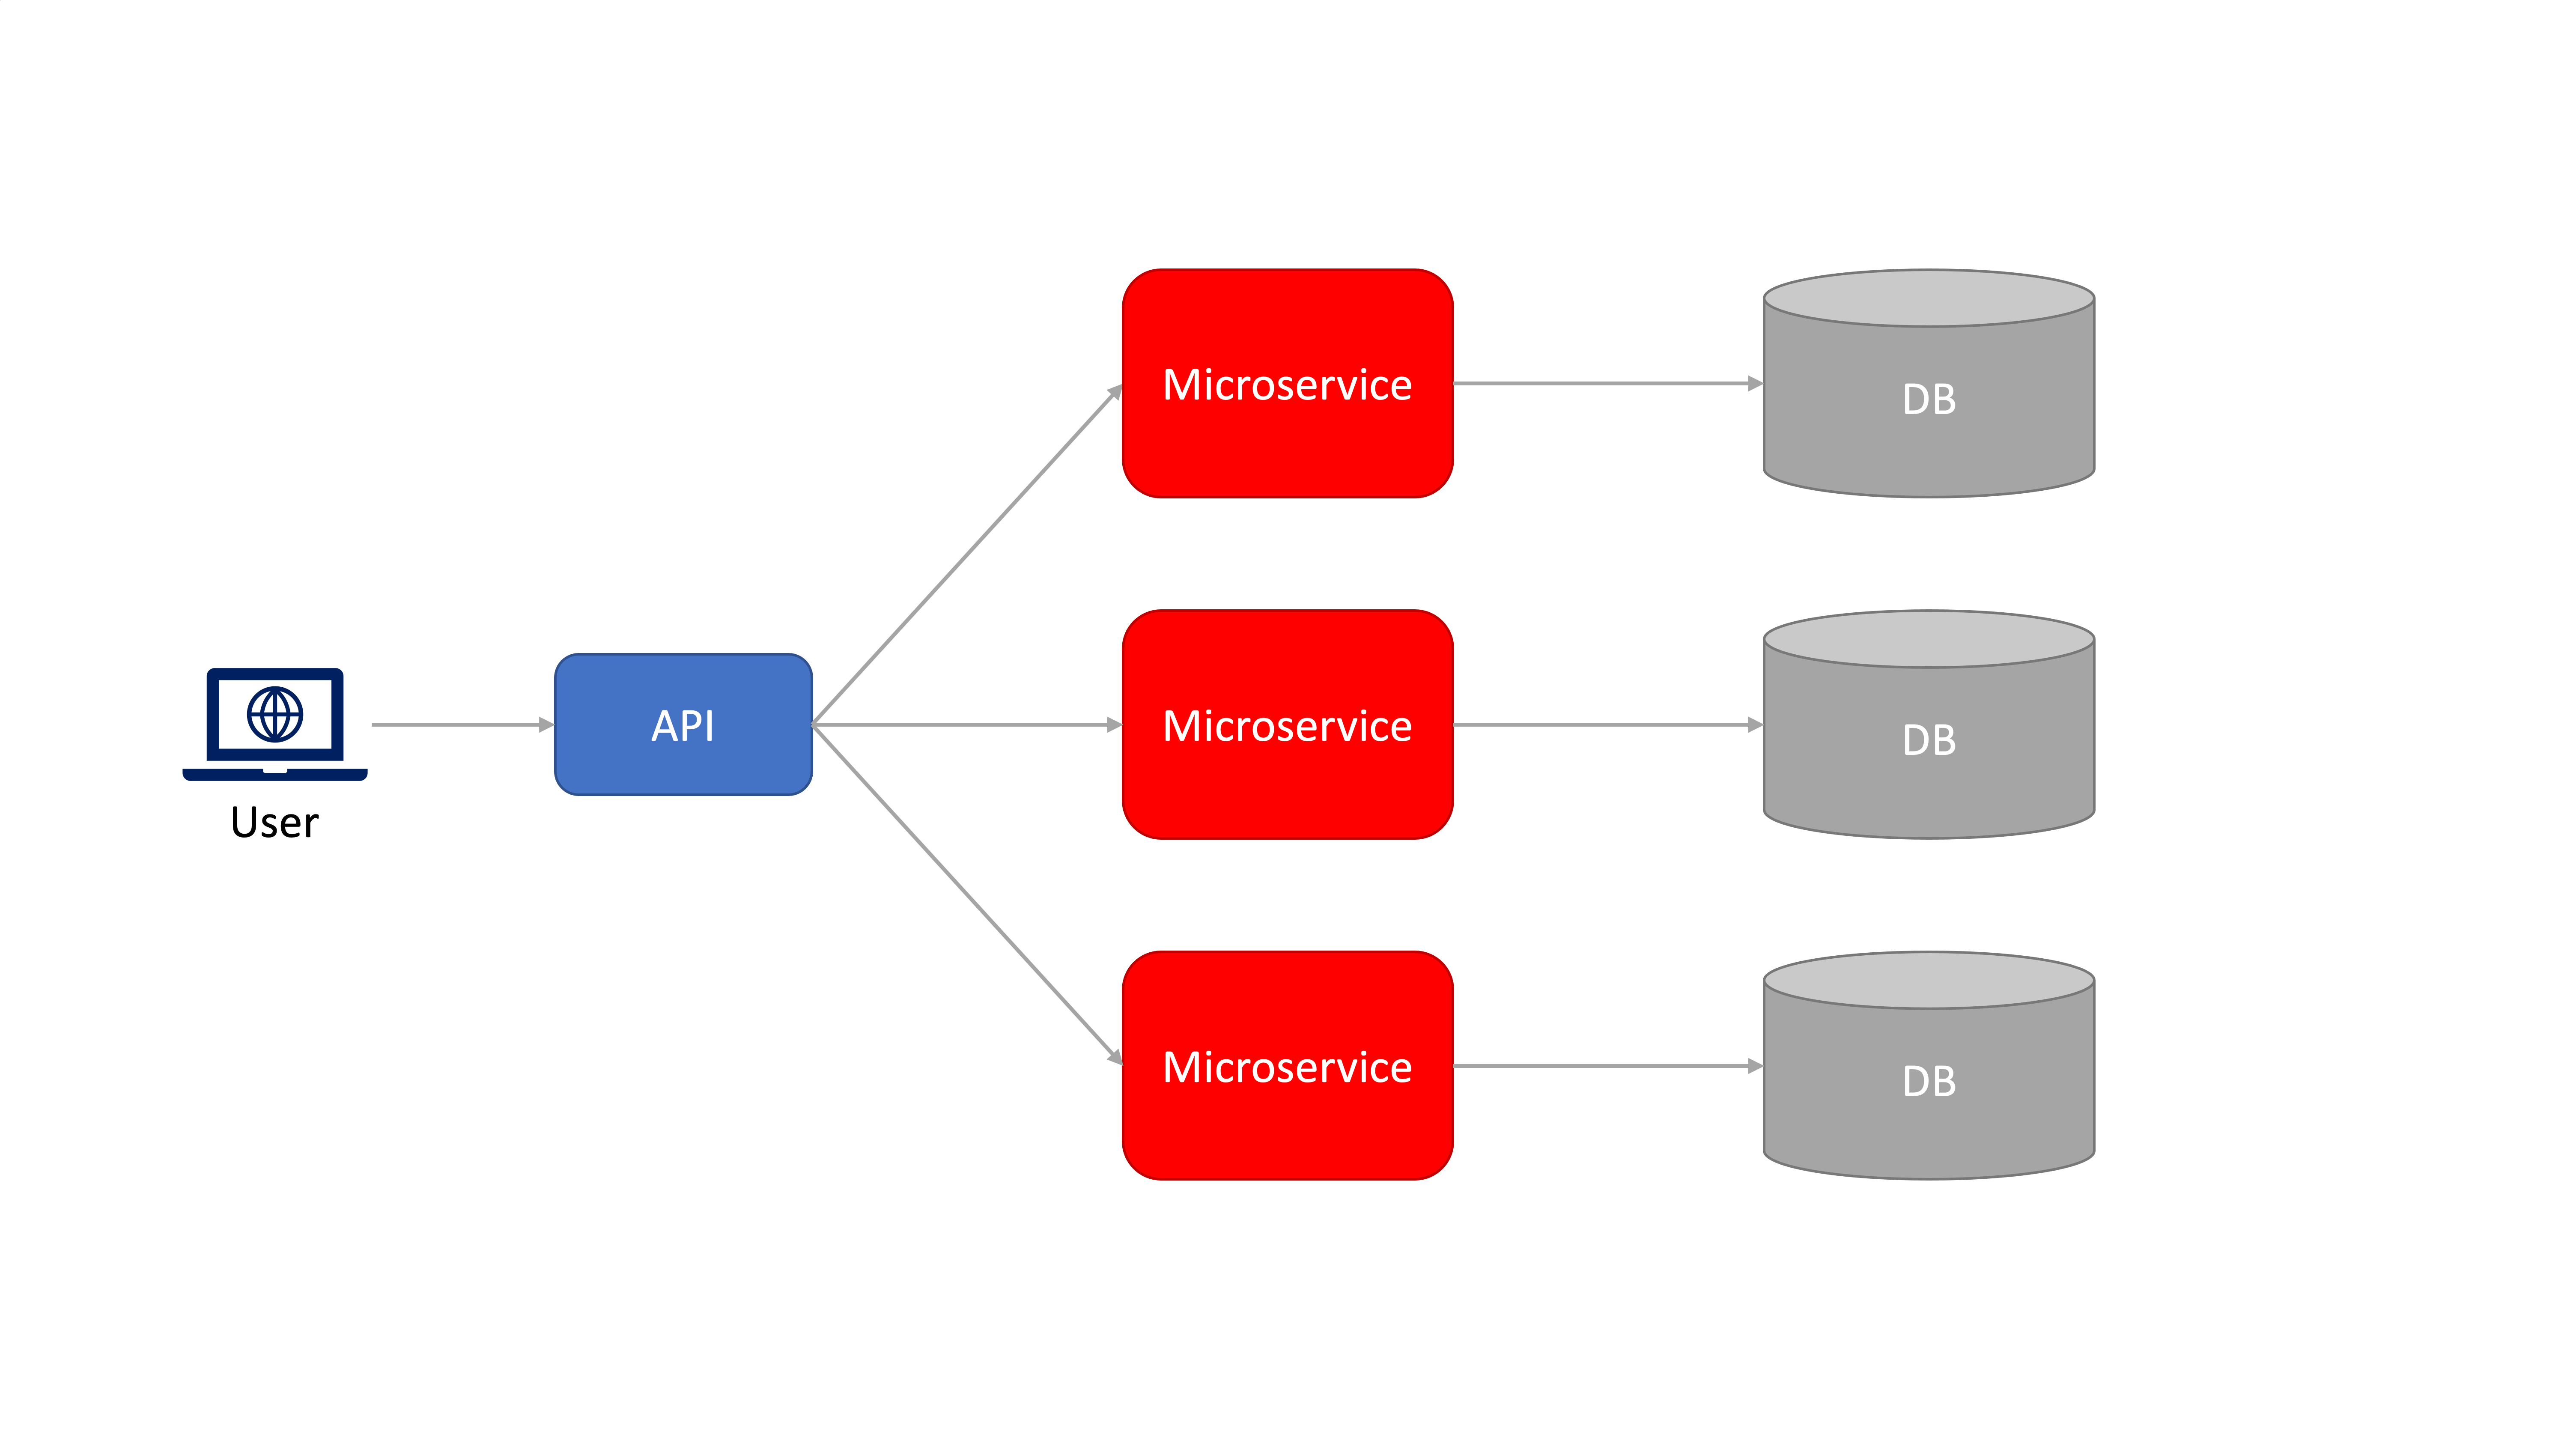
\includegraphics[width=0.65\textwidth]{microservice.png}
    \caption{Beispiel einer Microservice Architektur \cite[Nachbildung angelehnt an][S. 150]{Gos2020}}
    \label{fig:microservice}
\end{figure}

In Bezug auf Cloud-native Anwendungen bringen Microservices eine effizientere Skalierbarkeit mit sich, da jeder Service einzeln je nach Bedarf skaliert werden kann und nicht die komplette monolithische Anwendung skaliert werden muss \cite[Vgl.][]{Janssen2021}.

Die Entwicklung von Microservices hat außerdem den Vorteil, dass der Blick im Entwicklungsprozess separiert auf die einzelnen Services gelegt werden kann und der Entwickler somit nicht jederzeit den ganzen Monolithen im Auge haben muss, um zu verhindern, dass einzelne Funktionen sich gegenseitig beeinflussen \cite[Vgl.][]{Janssen2021}. \pagebreak

% In Bezug auf Cloud Native -> weil skalierbar (kleine Einheiten etc...)
% Fehlertoleranter
% Asynchrones Messaging (-> keine Fails, wenn Service ausfällt)

%title wird unter dem Bsp. abgedruckt
%caption wird im Verzeichnis abgedruckt
%label wird zum referenzieren benutzt, muss einzigartig sein.

% \begin{lstlisting}[caption=Code-Beispiel, label=Bsp.1]
% public class HelloWorld {
% 	public static void main (String[] args) {
% 		// Ausgabe Hello World!
% 		System.out.println("Hello World!");
% 	}
% }
% \end{lstlisting}

% %language ändert die Sprache. (Wenn nur eine Sprache verwendet wird, kann diese Sprache in einstellungen.tex geändert werden. Standardmäßig Java.)
% \begin{lstlisting}[caption=Python-Code, label=Python-Code, title=Titel des Python-Codes,language=Python]
% def quicksort(liste):
% if len(liste) <= 1:
% 	return liste
% pivotelement = liste.pop()
% links = [element for element in liste if element < pivotelement]
% rechts = [element for element in liste if element >= pivotelement]
% return quicksort(links) + [pivotelement] + quicksort(rechts)
% # Quelle: http://de.wikipedia.org/wiki/Python_(Programmiersprache)
% \end{lstlisting}

% \section{Verweis auf Code}
% Verweis auf den Code \autoref{Bsp.1}.\\
% und der Python-Code \autoref{Python-Code}.

% Zweite Erwähnung einer Abkürzung \ac{AGPL} (Erlärung wird nicht mehr angezeigt)